% Chapter Template

\chapter{Evaluation of Results and Discussion} % Main chapter title

\label{Chapter5} % Change X to a consecutive number; for referencing this chapter elsewhere, use \ref{ChapterX}

\lhead{Chapter 5. \emph{Evaluation of Results and Discussion}} % Change X to a consecutive number; this is for the header on each page - perhaps a shortened title

This chapter discusses the ability of an implementation of defeasible reasoning to model a construct in comparison with machine learning. The chapter presents and discusses the results of the experiment performed in the previous chapter. A comparative analysis of both techniques is performed using the evaluation techniques gathered in the literature review.

\section{Results}

The research question posed at the start of this project is focused on the ability of two techniques to represent a construct and make predictions based on this representation. The predictive capacity of the techniques is presented here. In order to determine how these new measures perform, the concurrent and convergent validity of the new values is calculated using existing measures of mental workload. 

\subsection{Predictive Capacity - Numeric}

In order to compare the predictive capacity of the approaches each technique was used to compute the value of an objective performance measure: time. The mean absolute error for time prediction was taken for each technique. In order to gather a wider comparison the size of the data used for training and testing was adjusted by varying the number of folds and percentage of split. Figure ~\ref{fig:mae_time} displays the results of the experiment. Immediately obvious in this graph is the poor performance of Artificial Neural Networks. According to \cite{silvert2000can} ANNs typically require large ammount of data for training. The performance of the ANN could be improved by pre-processing the data. It is also possible that the ANN has overfit the training data. This could be determined by evaluating the minimum description length of the model, however, this is is beyond the scope of the thesis as it is not possible to compare that measure with the knowledge based approach.

The performance of the machine learning algorithms vary dramatically. It is interesting to note that simple linear regression using one variable doesn't out perform the regression based on the non-expert knowledge base which is also based on one variable. Decision table, kstar and additive regression have error rates higher than the expert knowledge base. Decision table and kstar don't correlate well with time although additive regression performs nearly as well as the expert knowledge base. A linear regression outperforms all of the techniques and can predict task time with the strongest correlation. With the exception of linear regression, the machine learning techniques all show a large variability based on the amount of data that is available for training. KStar and additive regression are outperformed by linear regression. 

\begin{figure}[!h]
\centering
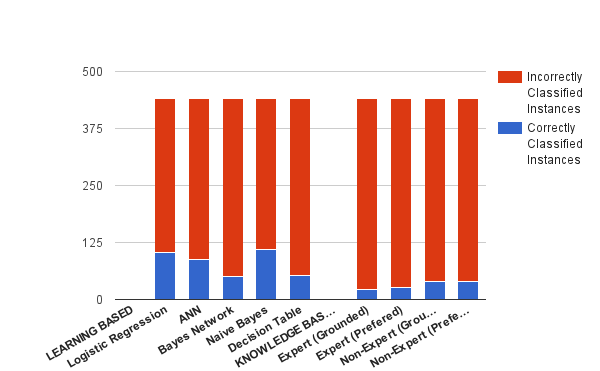
\includegraphics[width=\linewidth]{mae_time}
\caption{Mean Absolute Error for Time Prediction}
\label{fig:mae_time}
\end{figure}

Table ~\ref{tab:time_predictions_fold} and table ~\ref{tab:time_predictions_split} gives a breakdown of the results that provides more clarity than the previous figures. For different numbers of folds we can see that the regressions based on the expert's knowledge base perform best of all which validates the first hypothesis of the experiment. What is interesting is that the predictions based on the knowledge of the non-expert perform better than that of the expert for varying percentage of split. As the knowledge base of the non-expert contains fewer nodes it is possible that it weighs some variable heavily that contributes greatly to task time.

\begin{table}[!htbp]
\centering
\begin{tabular}{|c|c|c|c|}
\hline
                                &  10-fold & 20-fold & 40-fold \\ \hline
ANN                             & 137.238 & 126.9808 & 141.3834 \\
K Star                          & 93.6672 & 92.1658 & 91.1066 \\
Additive Regression             & 85.8072  & 83.5995  & 82.0641 \\
Regression                      & 80.8231 & 80.9963 & 80.2697 \\
Expert (Grounded Extension)     & 80.6007 & 80.5986 & 80.5241 \\
Expert (Prefered Extension)     & 80.4185 & 80.4475 &  80.3192 \\
Non-Expert (Grounded Extension) & 81.5565 & 81.6743 & 81.7295 \\
Non-Expert (Prefered Extension) & 81.5565 & 81.6743 & 81.7295 \\
\hline
\end{tabular}
\caption{Mean Absolute Error Using K-Fold Cross Validation}
\label{tab:time_predictions_fold}
\end{table}

\begin{table}[!htbp]
\centering
\begin{tabular}{|c|c|c|c|}
\hline
                                & 30\% Split  & 50\% Split  & 70\% Split \\ \hline
ANN                             & 163.7684 & 152.5288 & 147.3721 \\
K Star                          & 101.9482 & 93.8966 & 92.0756 \\
Additive Regression             & 93.3442  & 81.2395  & 87.8533 \\
Regression                      & 83.1717 & 80.868 & 83.589 \\
Expert (Grounded Extension)     & 81.0625 & 78.0558 & 78.7381 \\
Expert (Prefered Extension)     & 80.4185 & 80.4475 &  80.3192 \\
Non-Expert (Grounded Extension) & 79.5426 & 77.2909 & 79.9484 \\
Non-Expert (Prefered Extension) & 79.5426 & 77.2909 & 79.9484 \\
\hline
\end{tabular}
\caption{Mean Absolute Error Varying Percentage of Split}
\label{tab:time_predictions_split}
\end{table}

\subsection{Predictive Capacity - Task Membership}

A comparison of the techniques ability to predict task membership was also performed. The performance of each measure was evaluated simply using 10-fold cross validation. This was chosen as there are a larger number of evaluation metrics for classifiers that are being considered here than for the numeric prediction task. The first metric that is examined is the number of correctly and incorrectly classified instances which is shown in figure ~\ref{fig:classified}. This metric shows that ANN, Naive Bayes and Logistic Regression perform best in terms of correctly classified instances. This nullifies the hypothesis that the knowledge base of the expert predicts task membership better than machine learning. In this case the knowledge base of the expert actually performed worse than the knowledge base of the non-expert.

\begin{figure}[!h]
\centering
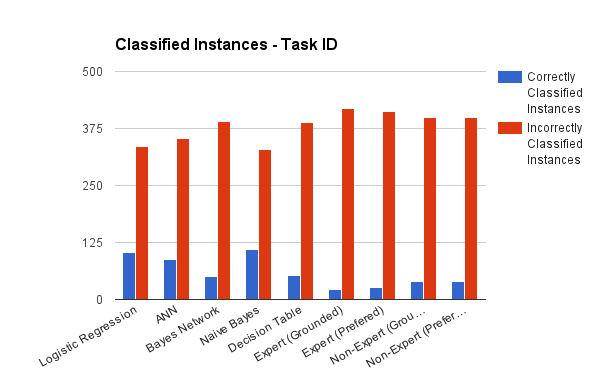
\includegraphics[width=\linewidth]{classified_instances}
\caption{Classified Instances - Task ID}
\label{fig:classified}
\end{figure}

By examining the precision and recall of the classifiers we can gain further insight into their performance. The best performing machine learning tasks have about the same precision and recall. We can see a large variation in the precision and recall of the expert and non-expert. The recall of the non-expert is higher than that of the expert resulting in a greater number of correctly classified instances.

\begin{figure}[!h]
\centering
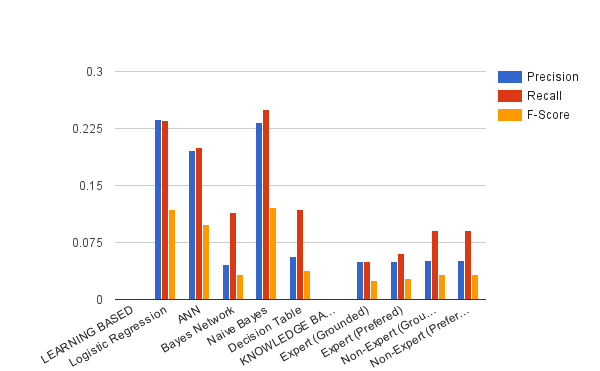
\includegraphics[width=\linewidth]{precision_recall_f-score}
\caption{Precision, Recall and F-Score}
\label{fig:precision_recall_f-score}
\end{figure}

The area under the ROC curve provides further clarification of the performance of the classifiers as it takes into account the number of false positives. We can see that while the non-expert may have classified more instances correctly, the expert's knowledge base provides a greater balance between true positives and false positives.  

\begin{figure}[!h]
\centering
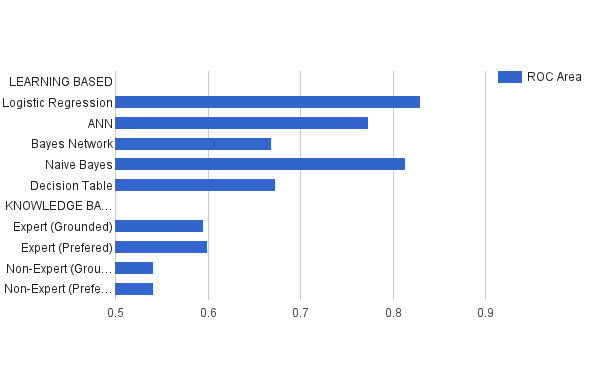
\includegraphics[width=\linewidth]{roc_area}
\caption{Area Under ROC Curve}
\label{fig:precision_and_recall}
\end{figure}

It is interesting that the machine learning approach was more effective in determining task membership than the defeasible reasoning approach. This could be because the tasks don't vary MWL strongly enough. Another possibility is that the knowledge bases are failing to take into account some aspect of mental workload that could determine task membership better.

\subsection{Concurrent Validity}

The concurrent validity of the defeasible constructs was measured by performing regressions against time (tables ~\ref{tab:ccurrent_time}). Time is an objective performance measure that is similar to MWL. The Pearson correlation provides an understanding of the performance of each knowledge base. The results show a much stronger correlation between the knowledge base of the expert and time than the knowledge base of the non-expert. This provides some confirmation that the implementation is modeling defeasible knowledge bases correctly as it is expected that the knowledge base of the expert should more accurately represent MWL that that of the non-expert. The preferred extension of the knowledge base of the expert performed better than the grounded extension. The preferred extension and the grounded extension of the non-expert were determined to be equivalent by the software and so show the same results.

\begin{table}[!htbp]
\centering
\begin{tabular}{c|c|c}
\hline
 & Grounded Extension & Preferred Extension\\ \hline
Expert & 0.3362        & 0.3414      \\
Non-Expert &  0.2046         & 0.2046  \\
\hline
\end{tabular}
\caption{Concurrent Validity - Pearson Correlation with Time}
\label{tab:ccurrent_time}
\end{table}

\subsection{Convergent Validity}

In order to determine how well the constructs actually modeled MWL the convergent validity of these measures was determined. The convergent validity was determined by computing the correlation of each measure with existing measures of MWL. These existing measures are the NASA Task Load Index and the Workload Profile. 

It can be seen that the expert's knowledge base correlates strongly with the other measures for MWL (table ~\ref{tab:corrmwlone}). There is a moderate correlation between other measures of MWL and and the non-expert's knowledge base. This strong correlation reinforces the belief that defeasible reasoning can accurately model a construct.

\begin{table}[!htbp]
\centering
\begin{tabular}{|c|c|c|c|}
\hline
                & NASA      &  WP        \\ \hline
expertGroundedExt  & 0.7233711 & 0.8593995 \\
expertPref1        & 0.7247067 & 0.8499664 \\
non-expertGroundedExt & 0.5518035 & 0.5648483 \\
non-expertPref1       & 0.5518035 & 0.5648483 \\
\hline
\end{tabular}
\caption{Pearson correlation of measures of MWL}
\label{tab:corrmwlone}
\end{table}

\section{Summary and Final Recommendations}

The results presented in this chapter were collected in order to test the designed hypotheses:

\begin{enumerate}
  \item The defeasible measure of a construct created by an expert is better at predicting objective performance values than machine learning approaches.
  \item The construct measure of an expert will have a high concurrent validity with objective measures related to the construct.
  \item The construct measure of an expert will have a high convergent validity with existing measures for the construct.
\end{enumerate}

\subsection{First Hypothesis}

The first hypothesis was examined by comparing the capacity of the techniques to make predictions of two objective values: task time and task ID.  

In the case of task time, the knowledge base of the expert proved to be the best for prediction. This supports the hypothesis. On the other hand the knowledge based approach performed worse for the prediction of task membership. These contradictory results require further investigation. The time prediction experiment should be further refined by including a greater number of knowledge bases and learners. A more statistically valid comparison of the task ID and MWL value could be performed, for example by examining the distribution of MWL values with respect to the task ID.

As the expert and non-expert knowledge bases perform similarly, it is difficult to tell why the approaches perform the way they do. It is possible that as regressions are performed, the use of one independent variable is more useful than using many. Future work might include a comparison between knowledge bases that use intentionally bad premises to model MWL and expert ones.

\subsection{Second Hypothesis}

The second hypothesis was examined by determining the concurrent validity of the measures of mental workload with time, an objective performance measure. It was found that the knowledge base of the expert had a statistically significant correlation with time, however, it was not a very strong one. This can be explained by considering the construct of MWL as a defeasible phenomenon. The time spent on a task could be high, however, the participant may not be very motivated or may be distracted. In this case the MWL would in fact be low. A short coming of machine learning is highlighted here. If we do not believe time to accurately model MWL in all cases we must create a new model. This would require an expert to apply labels to the data in a time consuming procedure.

\subsection{Third Hypothesis}

The third hypothesis was examined by determining the convergent validity of the measures of MWL with other existing measures of MWL: NASA-TLX and Workload Profile. It was found that the construct measure developed by the expert had a high convergent validity with existing measures of MWL. It was also found that the construct measure of the expert had a higher convergent validity than that of a non-expert. This reinforces our belief that the defeasible modeling of the construct is working effectively. Again, it should be pointed out that this modeling is not possible in supervised machine learning without applying labels to the data. An underlying flaw in this approach is that it is assumed that the existing measures correctly model the construct. These measures may be proven invalid in the future and so if such a system were to be adopted it is important to consider this. The accuracy of the diagnoses made by the knowledge based system are entirely influenced by the knowledge used. The system cannot automatically detect that the mappings from premises to conclusions are incorrect. On the other hand, it is hoped that through using the system and obtaining visual feedback a user might improve their understanding in their area of expertise.

\subsection{Recommendations}

These finding support the case for the implementation of defeasible reasoning as an alternative to learning based approaches. 

The main advantage of learning based systems is that the learning is automatic. If given enough data and enough computing power machine learning can tackle many problems well. However, the available data sets are often not comprehensive enough or representative of the wider picture. This can result in models that are too localised and unable to predict exceptional cases. Data often must be cleaned and labeled, a time consuming and expensive process. Knowledge based approaches offer and alternative to this. The results of the experiments suggest that knowledge based approaches offer a viable alternative for prediction. While the time to input a knowledge base is non-trivial, it is less than the time required for labeling in many cases.

One of the shortcomings of using convergent validity for assessment is that the existing measures of the construct must also model the construct accurately. This means that while in this particular instance we have shown a strong concurrent validity with existing constructs, this may not always be the case. In order to further verify that the system is working as intended more experiments need to be performed with a wider variety of knowledge bases and data sets. If it is then verified that the system works as intended it may then be used to develop alternative measures for constructs that deviate from previous measures. 

What has not been examined is the role that the system feedback could play in improving an expert's understanding. the machine learning techniques typically represent their findings as numeric and mathematical models. In the DR system it is possible to represent these visually. Comparing these representations and how helpful they are in assisting an expert could be the subject of future work.